\documentclass[12pt,letterpaper]{article}
\title{Problemas Semana 3}
\usepackage{amsmath}
\usepackage{amssymb}
\usepackage{siunitx}
\usepackage{float}
\usepackage{tikz}
\usepackage[american,RPvoltages,siunitx]{circuitikz}
\ctikzset{capacitors/scale=0.7}
\ctikzset{diodes/scale=0.7}
\usepackage{tabularx}
\newcolumntype{C}{>{\centering\arraybackslash}X}
\renewcommand\tabularxcolumn[1]{m{#1}}% for vertical centering text in X column
\usepackage{tabu}
\usepackage[spanish,es-tabla]{babel}
\usepackage{babelbib}
\usepackage{booktabs}
\usepackage{pgfplots}
\usepackage{hyperref}
\hypersetup{
    colorlinks=true,
    linkcolor=azulTEC,
    urlcolor=azulTEC,
    citecolor=azulTEC,
    pdftitle={\@title},
    pdfauthor={Juan J. Rojas},
    pdfsubject={Instituto Tecnológico de Costa Rica},
    pdfcreator={LaTeX Beamer con Tectonic}
}
\usepgfplotslibrary{units, fillbetween} 
\pgfplotsset{compat=1.18}
\usepackage{bm}
\usetikzlibrary{
    decorations.markings,
    calc,
    arrows, 
    arrows.meta,  
    shapes, 
    3d, 
    perspective
}
\renewcommand{\sin}{\sen} %change from sin to sen
\usepackage{bohr}
\setbohr{distribution-method = quantum,insert-missing = true}
\usepackage{elements}
\usepackage{enumitem}
\usepackage{geometry}  
\geometry{left=18mm,right=18mm,top=21mm,bottom=21mm,headheight=15pt}
\setlength\parindent{0pt} % Removes all indentation from paragraphs
\usepackage{fancyhdr}
\pagestyle{fancy}
\lhead{Problemas de apoyo: Electricidad I}
\rhead{\begin{picture}(0,0) \put(-110,0){
\includegraphics[width=40mm]{figures/logo.png}} \end{picture}}
\usepackage{titlesec}

\titleformat{\section}{\normalfont \Large \bfseries}
{Semana\ \thesection}{2.3ex plus .2ex}{} %% Text "Semana" is what you would like the section number to display with.

\titleformat{\subsection}[runin]{\normalfont \large \bfseries}
{Problema\ \thesubsection}{0pt}{} %% Text "Problema" is what you would like the section number to display with.


\newcommand{\asection}[2]{
\setcounter{section}{#1}
\addtocounter{section}{-1}
\section{#2}
}
\begin{document}
\input{shared/postamble}

\asection{9}{Capacitores e Inductores}

1.En condiciones cd. Halle la tensión en las terminales de los capacitores. 
 \begin{center}
     \begin{circuitikz}
         \draw
         (0,0)
           to[C,l=$C_1$,v=$V_1$ ]
         (0,3.5)
             to[short]
         (-3.5,3.5)
            to[R,l=\SI{40}{\ohm}] 
         (-3.5,0)
             to[short]
         (0,0)
         
         (4,3.5) 
            to[R,l=\SI{50}{\ohm}]
         (7,3.5)
           to[C,l=$C_2$,v=$V_2$ ]
         (7,0)
            to[short]
         (4,0)
             to[short]
         (0,0)
         
         (0,3.5)
             to[R,l=\SI{10}{\ohm}]
         (4,3.5)
             to[R,l=\SI{20}{\ohm}]
         (4,2)
            to[V,l=\SI{60}{\volt}, invert]
         (4,0)
         ;
     \end{circuitikz}
 \end{center}
 
 R/    \\[16pt]

2. Halle capacitancia equivalente entre las terminales a y b en el circuito (capacitancias existentes están en microfaradios).
 \begin{center}
     \begin{circuitikz}
         \draw
         (0,0)
           to[R,l=\SI{2}{\ohm}]
         (0,3.5)
              to[short]
         (0,6)
         (-0.1,3.7)node[left]{$v_1$}
         (0,3.5)
             
         (-3.5,3.5)node[left]{$a$}
            to[C, C=\SI{12}{\mu\farad},o-]
         (0,3.5)   
         (-3.5,0)node[left]{$b$}
             to[short,o-]
         (0,0)
         (0,6)
           to[C, C=\SI{80}{\mu\farad}]
         (4,6)
             to[short]
         (4,3.5) 
         (0,0)
            to[C, C=\SI{50}{\mu\farad}]
         (4,3.5)
            to[C, C=\SI{20}{\mu\farad}]
         (8,0)
         (8,3.5)
           to[C, C=\SI{10}{\mu\farad}]
         (8,0)
            to [short]
         (4,0)
             to[C, C=\SI{60}{\mu\farad}]
         (0,0)
        
         (0,3.5)
             to[C, C=\SI{40}{\mu\farad}]
         (4,3.5)
         (4.1,3.7)node[right]{$v_2$}
         (4,3.5)
             to[C, C=\SI{30}{\mu\farad}]
         (4,0)
         (4,3.5)
             to[short] 
         (8,3.5)
         ;
     \end{circuitikz}
 \end{center}
 R/  \\[16pt]

3. Suponiendo que los capacitores están inicialmente descargados, halle $V_o$ (t) en el circuito. 
 \\ 
 ver figura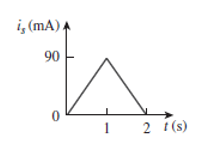
\includegraphics{figures/Capacitor cargado graf.PNG}
 \begin{center}
     \begin{circuitikz}
         \draw
         (0,0)
           to[I,I=$i_x$]
         (0,3.5)
             to[short]
         (0,6)
           to [short]
         (4,6)
            to[C, C=\SI{6}{\mu\farad}]
         (4,3) 
        
         (4,0)
            to[short, -o]
         (7,0)node[above]{$b$}
            to[short]
         (0,0)
    
         (4,3)
            to[C, C=\SI{3}{\mu\farad}]
         (4,0)
         (4,3)
             to[short, -o]
         (7,3)node[above]{$a$}
            to[open,v=$V_o$(t),invert]
         (7,0)
         ;
     \end{circuitikz}
 \end{center}

 
 R/   No\\[16pt]

4. La corriente que circula por un inductor de 40 mH es 
    \(
    i(t)=
    \begin{cases}
    0, & t<0,\\
    t e^{-2t}\,\mathrm{A}, & t>0.
    \end{cases}
    \)

halle la tensión v(t)
\\[16pt]

5. Obtenga el equivalente de Thevenin en las terminales a-b del circuito que aparece. (Tenga en cuenta que por lo general no existen este tipo de circuitos cuando hay inductores y capacitores)

 \begin{center}
     \begin{circuitikz}
         \draw
         (0,0)
           to[V,V=\SI{45}{\volt}]
         (0,5)
             to[short]
         (0,6)
           to [short]
         (4,6)
            to[C, C=\SI{5}{\farad}]
         (4,3) 
        
         (4,0)
            to[short, -o]
         (7,0)node[above]{$b$}
            to[short]
         (0,0)
    
         (5,3)
            to[C, C=\SI{2}{\farad}]
         (5,0)
         (4,3)
            to [short]
         (2.5,3)
            to[C, C=\SI{3}{\farad}]
         (2.5,0)
        
         (4,3)
             to[short, -o]
         (7,3)node[above]{$a$}
            
         ;
     \end{circuitikz}
 \end{center}
R/
\\[16pt] 

6. En condición cd en estado estacionario, halle i y v en el circuito.
 \begin{center}
     \begin{circuitikz}
         \draw
         (0,0)
           to[R,l=\SI{30}{\kilo\ohm}]
         (0,3.5)
             to[short]
         (-3.5,3.5)
             to[I,l=\SI{5}{\milli\ampere},invert]
         (-3.5,0)
             to[short]
         (0,0)
         
         (4,3.5) 
            to[R,l=\SI{20}{\ohm}]
         (7,3.5)
           to[R,l=\SI{20}{\kilo\ohm}]
         (7,0)
            to[short]
         (4,0)
             to[short]
         (0,0)
         
         (0,3.5)
             to[L, L=\SI{2}{\milli\henry}, i>^=$i$]
         (4,3.5)
             to[C,C=\SI{6}{\mu\farad},v=$V$]
         (4,0)
         ;
     \end{circuitikz}
 \end{center}
R/
\\[16pt]

7. Un inductor de 100 mH se conecta en paralelo con un resistor de 2$\si{\kilo\ohm}$. La corriente por el inductor es i(t)=50e$^{-400}$ mA. 
a) Halle la tensión $V_L$ en el inductor.
b) Halle la tensión $V_R$ en el resistor.
c) ¿Es $V_R$(t) + $V_L$(t) =0?
d) Calcule la energía en el inductor en t=0.\\[16pt]
 
8. La corriente que circula por un inductor de 12 mH es 4 sen(100t) A. Halle la tensión en el inductor en 0<t<$\pi$/200s, y la energía almacenada en t=$\pi$/200 s.\\[16pt] 

9.El interruptor ha estado ha estado mucho tiempo en la posición A. En t=0 se mueve de la posición A a la B. El interruptor es del tipo sin punto muerto, así que no hay interrupción en la corriente del inductor. Halle:\\
a) i(t) para t<0.\\
b) v inmediatamente después de que el interruptor se ha movido a la posición B.\\
c)v(t) mucho después de que el interruptor esta en la posición B.
\begin{center}
    \begin{circuitikz}[scale=0.8]\draw
            (0,2.5)  node[spdt, rotate = 90, yscale = -1, anchor=in] (Sw) {}
            (Sw.in) 
                to [L, L=\SI{0.5}{\henry}, voltage shift=3]
            (0,1) --  (0,0)
            (Sw.out 2) |- (-1,4) to [R,l=\SI{4}{\ohm},o-] (-4,4)
                to[V, v_=\SI{12}{\volt}, invert]
            (-4,0)
            (Sw.out 1) |- (1.5,4) to[short,o-] (3,4)
                to[R,R=\SI{5}{\ohm}]
            (3,0) to[short,-o] (1.5,0) to[short,-o] (-1,0) -- (-4,0)
            (1.5,4)
                
            (1.5,0)
            (3,4)
                to[short]
            (6,4)
            (6,0)
                to[I, l=\SI{6}{\ampere}, invert]
            (6,4)
            (6,0)
                to [short]
            (3,0)
            (-0.7,3.2)node[above]{$A$}
            (0.7,3.2)node[above]{$B$}
            ;
        \end{circuitikz}
\end{center}

10. Considere el circuito. Dado que v(t)=12e$^{-3t}$mV para t>0 e $i_1$(0)=-10 mA, Halle:\\
a) $i_2$(0)\\
b) $i_1$(t) e $i_2$(t).\\
 \begin{center}
     \begin{circuitikz}
         \draw
         
         (0,3.5)
           to[L,L=\SI{20}{\milli\henry}, i^=$i_1$(t)]
         (0,0)
             
         (-3.5,3.5)node[left]{$a$}
            to[L, L=\SI{25}{\milli\henry},o-]
         (0,3.5)   
         (-3.5,0)node[left]{$b$}
             to[short,o-]
         (0,0)
            
         (0,3.5)
             to[short]
         (4,3.5)
             to[L, L=\SI{60}{\milli\henry}, i^=$i_2$(t)]
         (4,0)
            to [short]
         (0,0)
        (-3.5,3.5)
            to[open,v=$V$(t)]
        (0,0)
         ;
     \end{circuitikz}
 \end{center}
R/
\\[16pt]

11. Considere el circuito. Halle:\\
a) $L_eq$, $i_1$(t) e $i_2$ si $i_s$= 3e$^{-t}$ mA\\ 
b) $V_o$(t)\\
c) La energía almacenada en el inductor de mH en t= 1 s.\\ 
 \begin{center}
     \begin{circuitikz}
         \draw
         
         (0,3.5)
           to[L,L=\SI{20}{\milli\henry}, i^=$i_1$, v=$V_0$]
         (0,0)
             
         (-3.5,3.5)node[left]{$a$}
            to[short]
         (0,3.5)   
         (-3.5,0)
             to[short]
         (0,0)
            
         (0,3.5)
             to[short]
         (4,3.5)
             to[L, L=\SI{4}{\milli\henry},i^=$i_1$]
         (4,2)
            to[L, L=\SI{6}{\milli\henry}]
         (4,0)
            to [short]
         (0,0)
        (-3.5,3.5)
            to[I, l=$i_s$, invert]
        (-3.5,0)
        ;
        \draw[thick] (-2.2,-1)node[right]{$L_{eq}$} -- (-2.2,1);
        \draw[thick,-latex] (-2.2,1) -- (-1.2,1);
     \end{circuitikz}
 \end{center}
 
 R/
 \\[16pt]




\end{document}